\documentclass[a4paper, 14pt]{extarticle}

% Configuration {{{
\usepackage[utf8]{inputenc}
\usepackage[T2A]{fontenc} % T1 for English
\usepackage[english, russian]{babel}

\usepackage{enumitem}
\setlist{nolistsep}
\usepackage{mathtools}
\usepackage{xcolor}
\definecolor{dimblue}{HTML}{1010aa}
\usepackage[
	colorlinks=true, 
	allcolors=dimblue
]{hyperref}
\usepackage[
	vmargin=1in,
	hmargin=1in
]{geometry}
\linespread{1.3}
\usepackage{indentfirst}
\usepackage{graphicx}
\usepackage[multidot]{grffile}
\usepackage[labelsep=period]{caption}
\usepackage{subcaption}

\hypersetup{
	pdfauthor=Kerim Guseynov,
	pdftitle=Supernovae Explosions,
}

\def\M{\mathrm{M}_\odot}
% }}}

\begin{document}

% Title Page and Table of Contents {{{
\thispagestyle{empty}

\begin{center}
	\small
	\textsc{Московский государственный университет имени М.\,В.~Ломоносова}
	\\\vskip-1.7\baselineskip\null\hrulefill\null\vskip-.3\baselineskip
	\textsc{Кафедра общей ядерной физики}
\end{center}

\vfill

\begin{center}
	{\Large\textbf{Взрывы сверхновых}}
\end{center}

\vskip.3\baselineskip

\begin{flushright}
	Выполнил студент 113М группы \\
	Гусейнов Керим Демирович

	Под руководством \\
	доцента Третьяковой Татьяны Юрьевны
\end{flushright}

\vfill

\begin{center}
	Москва --- 2021
\end{center}

\clearpage

\tableofcontents

\clearpage
% }}}

\section{Введение}
% {{{

Появление философии, а затем и физики, во многом обязано прекрасному 
и загадочному ночному небу. Различные модели устройства Вселенной 
формировались в разные эпохи и сопутствовали мыслителям во всем. 
С появлением более формальных подходов и накоплением экспериментальных 
наблюдений, стало возможным аргументированно строить модели и описывать 
Вселенную, подчиняющуюся известным законам.
%
Развитие фундаментальной физики в конечном итоге привело к существенно 
более глубокому пониманию процессов в микромире, открытию гигантского 
массива частиц и еще большему интересу к теме эволюции Вселенной.

Физика частиц на данный момент является наиболее фундаментальной частью 
физики, напрямую взаимодействующей с экспериментом. Касательно развития 
Вселенной, физика частиц затрагивает самые ранние мгновения и самые 
базовые свойства их ``конечного состояния'', которое затем вступает 
в область, описываемую ядерной физикой. Среди этих свойств одним из 
наиболее значимых для нуклеосинтеза является наличие реликтового 
излучения, образовавшегося в результате аннигиляции основного объема 
вещества и антивещества, возникшего в ходе Большого взрыва. При 
дальнейшем расширении Вселенной и завершении первичного нуклеосинтеза, 
осталось лишь несколько видов ядер, самые многочисленные из которых -- 
водород и гелий. Распределяясь по пространству, они долгое время 
скапливались вокруг мест случайных неоднородностей под действием одной 
лишь гравитации. Образовав вещество достаточной плотности и температуры, 
ядра начали вступать в реакции слияния, вновь запуская нуклеосинтез, 
только теперь не во всей Вселенной, а внутри гигантских облаков -- 
звезд первого поколения.

Нуклеосинтез в звездах приводит к образованию множества разнообразных 
ядер и изотопов, которые можно наблюдать практически из любой точки 
Вселенной. Выявление более тонких закономерностей нуклеосинтеза 
и условий его протекания позволяет проверять современные методы описания 
ядерных реакций и представления о развитии Вселенной.

Сверхновые, в свою очередь, являются последним этапом эволюции самых 
массивных звезд (сверхновые II типа), а также могут представлять 
завершающий этап жизни остатков некоторых более легких звезд (сверхновые 
Ia типа). В обоих случаях происходит колоссальный выброс энергии 
и вещества в космическое пространство. Светимость одной единственной 
сверхновой сопоставима со светимостью целой галактики. Изучение взрывов 
сверхновых позволяет описать эволюцию галактик в целом и, в частности, 
образование планет и систем, аналогичных солнечной.

% }}}

\section{Общая эволюция звезд}
% {{{

Для лучшего понимания процессов, происходящих при взрывах сверхновых, 
необходимо хотя бы в общих чертах представлять структуру звезд и их 
эволюцию.

В результате взрывов звезд первого поколения в космос был выброшен набор 
прежде не существовавших ядер, без которых не возникло бы комет, планет 
и многих других небесных тел. Кроме того, попадая в новые звезды, эти 
элементы открывают дополнительные каналы протекания ядерных реакций 
в экстремальных условиях центров звезд. В связи с этим, полезнее будет 
описать эволюцию звезд второго поколения, параллельно выделяя 
особенности, присущие лишь им.

Как уже было сказано, звезды представляют собой гигантские массы 
преимущественно легких ядер, собравшихся вокруг центра неоднородности 
посредством гравитационного взаимодействия. Если масса вещества 
оказывается слишком мала для запуска реакции синтеза водорода, звезда не 
зажигается, не испускает энергичные фотоны и называется коричневым 
карликом. Дальнейшая эволюция такой звезды обусловлена лишь внешними 
источниками вещества.

При достижении массы исходного вещества значения более $0.08\,\M$ 
становится возможным горение водорода, протекающее параллельно в двух 
циклах. Один из них, называемый $pp$-циклом, не задействует других ядер, 
кроме водорода, образуя из них изотопы водорода и гелия, а также $^7$Be 
и $^7$Li. Второй цикл, называемый CNO-циклом, проходит в присутствии 
$^{12}$C, действующего в роли катализатора, и приводит к образованию 
$^4$He. Реакции обоих циклов требуют больших температур и проходят 
только в центре звезды, то есть звезда сохраняет толстый слой водорода 
вокруг центра. Когда запасы водорода в центре исчерпаны, звезда 
сжимается под действием гравитации и при наличии необходимой массы 
запускает горение водорода.

Горение водорода запускается в звездах с массой более $0.3\,\M$ и менее 
разнообразно по сравнению с водородом. Слияние трех альфа-частиц и их 
последовательное присоединение к получающимся ядрам приводит 
к образованию симметричных четно-четных ядер от $^{12}$C до $^{24}$Mg, но 
преимущественно $^{12}$C и $^{16}$O. Кроме того, в массивных звездах 
второго поколения на этом этапе уже начинается образование нейтронов. 
Одновременно с процессами в центре звезды, горение водорода переходит на 
периферию, в результате чего радиус возрастает на порядки, и звезда 
превращается в красный гигант. В итоге этой стадии звезда приобретает 
слоистую структуру, где внешний слой занят водородом, промежуточный -- 
гелием, а центр -- углеродом и кислородом, а для более массивных звезд 
еще и неоном и магнием.

После этого, если масса звезды превышает $5\,\M$, начинается горение 
углерода, затем неона и затем кислорода. Такой порядок обусловлен 
кулоновским барьером реакций. Горение углерода образует неон, магний 
и натрий. Неон в основном расщепляется на кислород и гелий, поскольку 
гамма-кванты в центре звезды уже имеют большую энергию. Слияние ядер 
кислорода образует кремний, фосфор и серу. Вылетающие в реакциях 
альфа-частицы, протоны и нейтроны быстро взаимодействуют с ядрами 
и существенно увеличивают набор возможных каналов. Больше всего на этой 
стадии образуется кремния, который занимает центральную часть звезды, 
добавляя таким образом четвертый слой.

Горение кремния возможно только в самых массивных звездах, изначальная 
масса которых составляет больше $25\,\M$. В этом случае в центре звезды 
протекают все реакции синтеза, завершающиеся на железе, удельная энергия 
связи которого максимальна. Горение кремния не может проходить в виде 
слияния, как это было с другими ядрами, из-за существенного кулоновского 
барьера. Вместо этого, большие температуры и энергичные гамма-кванты 
приводят к выбиванию протонов, нейтронов и альфа-частиц из кремния. 
Реакции этих частиц с ядрами чрезвычайно разнообразны, но глобально 
приводят к образованию ядер между $^{28}$Si и $^{56}$Fe. На этой стадии 
звезда достигает наибольших размеров, а реакции синтеза еще активнее 
протекают на периферии. В результате возникает богатая слоистая 
структура, представленная на рисунке~\ref{fig:layers.25M}. Кроме того, 
в таких звездах соблюдаются условия, необходимые для протекания 
s-процесса, рождающего тяжелые стабильные ядра.

\begin{figure}% {{{
	\centering
	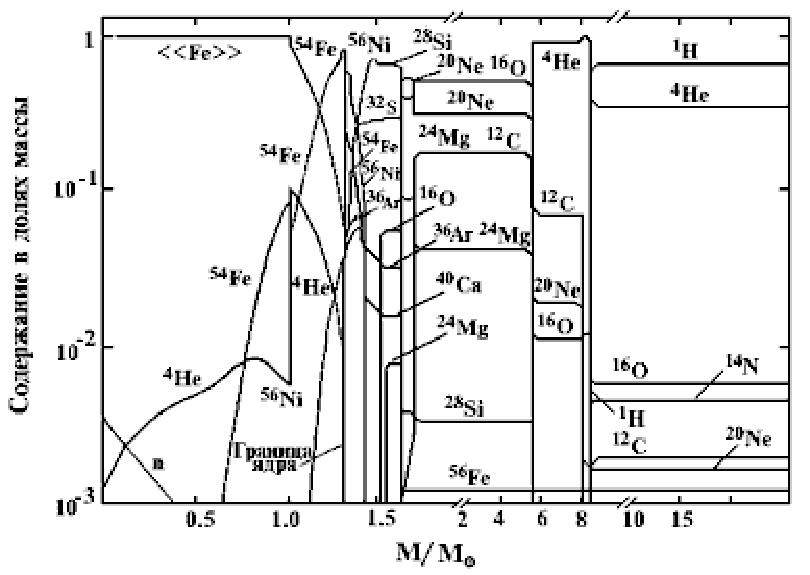
\includegraphics[width=.7\textwidth]{figures/nsf28.gif.pdf}
	\caption{Радиальная структура звезды с массой $25\,\M$ в результате 
	всех реакций синтеза.}
	\label{fig:layers.25M}
\end{figure}% }}}

% }}}

\section{Последние этапы эволюции звезд}
% {{{

\subsection{Легкие звезды}
% {{{

В процессе эволюции звезды теряют существенную часть своей массы, 
выбрасывая вещество в космос. Это происходит потому что при переходе 
реакций синтеза в оболочку звезды, условия в ней оказываются не такими 
же, как были на соответствующей стадии в центре. Во-первых, гравитация 
действует не так же, а во-вторых различные слои сильнее перемешиваются, 
позволяя многим реакциям протекать интенсивнее.

Для более легких звезд эволюция может закончиться на кремнии, кислороде 
и углероде, или даже на гелии. Случай гелия выделяется, поскольку выброс 
энергии при горении водорода сравнительно мал, а время выгорания всего 
водорода в звезде при массе, недостаточной для слияния гелия, 
значительно превышает возраст Вселенной. Считается, что существующие на 
данный момент гелиевые белые карлики образовались в двухзвездных 
системах из-за того, что сосед перетянул на себя их водородную оболочку. 
В остальных случаях предпоследним этапом является существенное 
увеличение радиуса и сброс части оболочки, обусловленные как раз 
перемещением нуклеосинтеза на периферию. Этот процесс идет сравнительно 
медленно, но завершается быстрым сбросом оставшейся оболочки 
и обнажением ядра звезды. Дальнейшему сжатию противостоит давление 
вырожденного электронного газа в ее объеме.

Касательно механизма быстрого сброса оболочки устоявшегося мнения нет, 
но лучше всего этот процесс понят для белых карликов, состоящих из 
кислорода и углерода. Особенность горения гелия, тройного альфа-процесса, 
в том, что оно чрезвычайно сильно зависит от температуры и вследствие 
этого неустойчиво. При небольшом увеличении температуры существенно 
возрастает скорость реакции, что вновь увеличивает температуру, 
и процесс приобретает взрывообразный характер. Кроме того, 
в несферических звездах могут возникать колебания, сопровождающиеся 
интенсивным испусканием вещества. Выброс вещества не всегда происходит 
симметрично. Например, на рисунке~\ref{fig:red.rect} представлена 
прямоугольная планетарная туманность, выброшенная красным гигантом. 
Помимо анизотропии, эта туманность состоит из отчетливых волн вещества, 
обусловленных, вероятно, колебаниями оболочки.

\begin{figure}% {{{
	\centering
	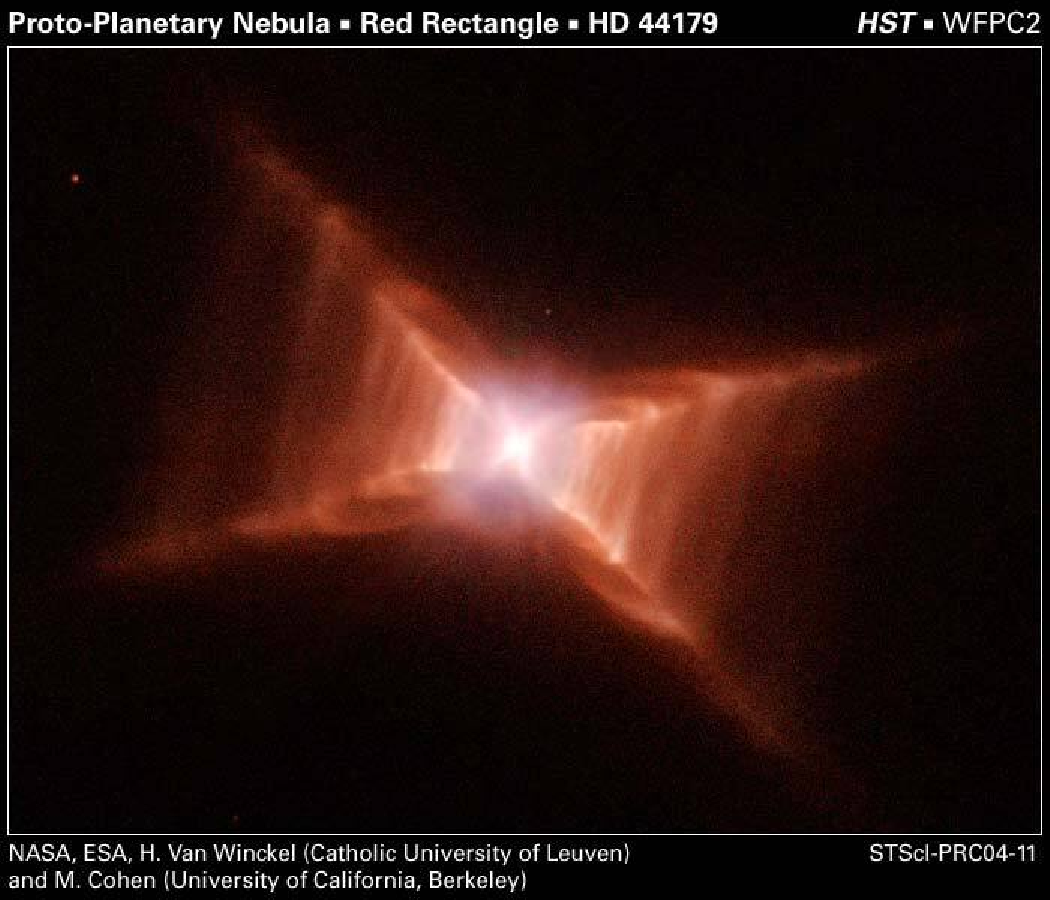
\includegraphics[width=.5\textwidth]{figures/Proto-Planetary.Nebula.HD44179.large.jpg.pdf}
	\caption{Протопланетарная туманность HD 44179: асимметричный выброс газопылевой материи красным гигантом}
	\label{fig:red.rect}
\end{figure}% }}}

После сброса оболочки звезда представляет собой лишь ядро, называемое 
белым карликом, путешествующее по галактике. Чаще всего встречаются 
белые карлики, состоящие из углерода и кислорода. Если белый карлик 
встречается с другой звездой, то есть оказывается в двухзвездной 
системе, вещество со второй звезды перетекает на белый карлик под 
действием его мощного гравитационного поля. Масса белого карлика может 
в конце концов достигнуть $1.4\,\M$, что оказывается несколько меньше 
предела гравитационного коллапса, и запустить реакции слияния углерода 
и кислорода в центре, а затем и в остальном объеме, подобно взрывной 
волне. Особенность протекания реакций в белых карликах в том, что их 
размер обусловлен давлением вырожденного газа электронов. Поэтому, по 
сравнению с центром звезды, резкое выделение энергии и увеличение 
температуры не приводит к сильному расширению, и реакция проходит 
существенно быстрее. Благодаря чрезвычайно высоким температурам, кремний 
испытывает прямое слияние вместо е-процесса, встречающегося в тяжелых 
звездах. Таким образом, в новообразовавшемся ядре звезды появляются 
нуклиды железного максимума, включая радиоактивные изотопы, наиболее 
многочисленным из которых оказывается $^{56}$Ni. Распадаясь по 
$e$-захвату с периодом 6 дней, $^{56}$Ni превращается в $^{56}$Co 
в возбужденном состоянии с энергией 1.72~МэВ. Кобальт испускает каскад 
гамма-квантов с энергиями от 0.16 до 1.56~МэВ и оказывается в основном 
состоянии. Гамма-кванты рассеиваются, поглощаются и разогревают ядро 
и оболочку, делая звезду менее плотной и открывая возможность вылета 
большему числу фотонов. Дальнейший распад самого кобальта происходит 
посредством $e$-захвата или $\beta^+$-распада с периодом полураспада 77 
дней. Ядра железа образуются в многочисленных возбужденных состояниях 
вплоть до 4.2~МэВ и испускают каскады гамма-квантов. Появление позитрона 
в результате $\beta^+$-распада $^{56}$Co также приводит к образованию  
гамма-квантов. Более подробно процессы распада ядер изображены на 
рисунке~\ref{fig:NiCoFe}.

\begin{figure}% {{{
	\centering
	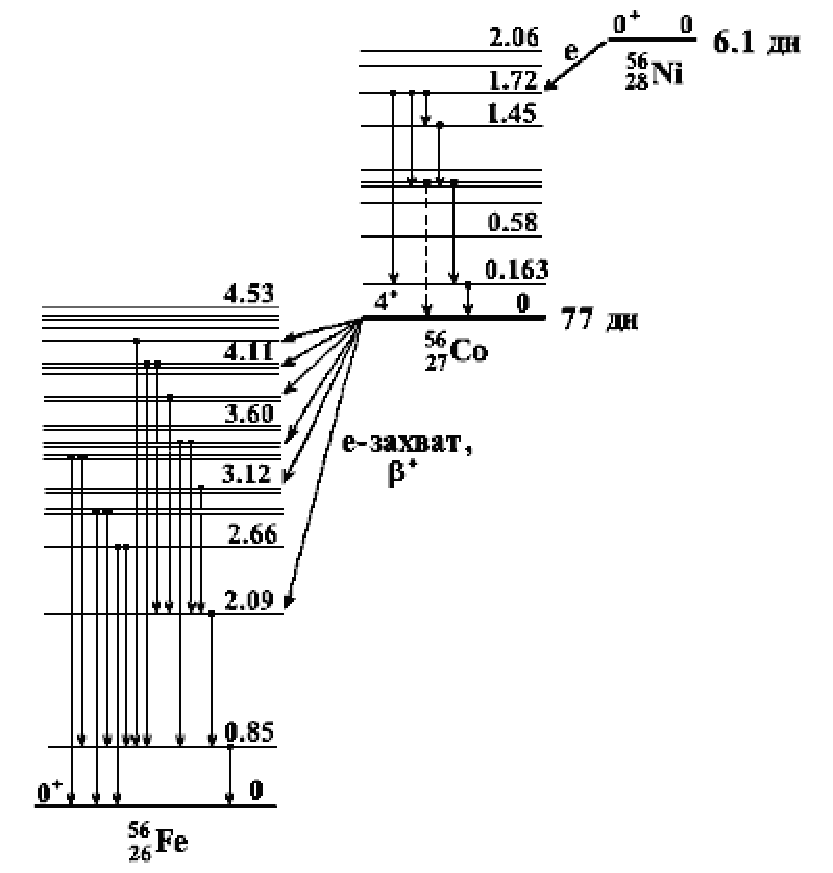
\includegraphics[width=.5\linewidth]{figures/nsf33.gif.pdf}
	\caption{Схема уровней и распадов ядер $^{56}$Ni, $^{56}$Co и $^{56}$Fe.}
	\label{fig:NiCoFe}
\end{figure}% }}}

Зарегистрированная в 1987 году сверхновая SN~1987A содержит некоторые 
характеристики, присущие взрывам сверхновых типа~Ia. Во-первых, 
излучение содержит линии $^{56}$Co. Во-вторых, в первые дни наблюдается 
рост интенсивности, поскольку все больше гамма-квантов кобальта вылетает 
за пределы звезды по мере расширения оболочки и уменьшения ее плотности. 
Сама же сверхновая SN~1987A принадлежит типу~II. Пересечение свойств 
обусловлено наличием тех же самых изотопов ядер железного максимума во 
всех сверхновых.

\begin{figure}[t!]% {{{
	\centering
	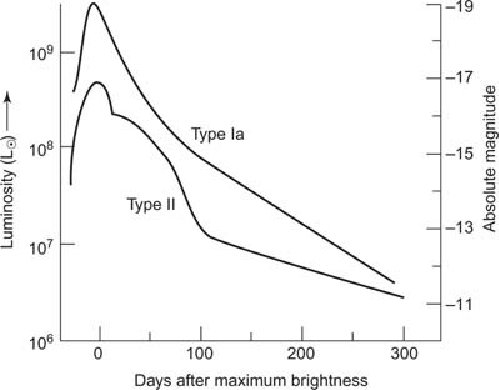
\includegraphics[width=.6\linewidth]{figures/23429.jpg.pdf}
	\caption{Светимости сверхновых типа~Ia и~II.}
	\label{fig:lumi}
\end{figure}% }}}

Для внешнего наблюдателя основным отличием между взрывами сверхновых 
различных типов является форма зависимости светимости от времени. На 
самом деле определяющим фактором в классификации является наличие или 
отсутствие линий определенных веществ в спектре, но мы обратимся к этому 
чуть позже. Светимости сверхновых типа~Ia и~II изображены на 
рисунке~\ref{fig:lumi}. Описанный процесс взрыва сверхновой типа~Ia 
предоставляет уникальную возможность, поскольку кривая светимости в этом 
случае должна быть одинаковой для всех сверхновых этого типа вне 
зависимости от того, где и как произошли взрывы. Вследствие этого, 
измеряя поток фотонов, можно определить на каком расстоянии произошел 
взрыв и вместе с этим на каком расстоянии находится соответствующая 
галактика. Однако такой тип сверхновой может также образовываться 
в столкновениях двух белых карликов~\cite{dwarf-collision} и в таком 
случае будет иметь меньшую интенсивность. Эта проблема для данного 
стандарта при измерениях расстояний во Вселенной, однако, сильно 
смягчается тем фактом, что вероятность столкновения белых карликов 
ощутима лишь в самых старых эллиптических галактиках.

Кроме сверхновых типа~Ia и~II существуют еще и типы~Ib и~Ic, но тип~Ia 
остается единственным, происходящим при участии белых карликов. Все 
остальные обусловлены гравитационным коллапсом тяжелых звезд. Типы~Ia,~b 
и~c объединены одной цифрой~I поскольку у них всех отсутствуют линии 
водорода. Дело в том, что сверхновая типа~Ib представляет собой коллапс 
тяжелой звезды, лишенной водородной оболочки, а типа~Ic -- лишенной как 
водородной, так и гелиевой оболочек. Подобные звезды могут появляться 
в двухзвездных системах, где компаньон перетянул на себя соответствующие 
слои массивной звезды.

% }}} Light Stars

\subsection{Тяжелые звезды}
% {{{

Самые тяжелые звезды имеют другой путь и, самое главное, результат 
эволюции. После образования в центре звезды ядер железного максимума 
весь запас ядерной энергии исчерпан. Звезда сжимается под действием 
гравитации и реакций синтеза во внешних слоях, поднимая температуру 
в центре до таких значений, что ядра железного пика расщепляются  
обратно на легкие ядра, альфа-частицы, протоны и нейтроны. Ядро звезды 
начинает поглощать энергию. Появившиеся легкие ядра, альфа-частицы 
и нуклоны вступают в реакции с другими ядрами. Сжатие также приводит 
к увеличению энергии электронов и открытию множества каналов 
$e$-захвата, при этом ядро звезды обогащается нейтронами, а температура 
вновь уменьшается. Таким образом, гравитационное сжатие звезды уже не 
приводит к повышению температуры в центре, и гравитация беспрепятственно 
продолжает сжимать звезду, а вещество падает с большой скоростью.  
Учащение столкновений приводит к существенному ускорению реакций синтеза 
в оболочке. В то же время, дальнейшее уплотнение центра звезды 
провоцирует еще более интенсивную нейтронизацию. Возникает огромный 
поток нейтрино, уносящий большую часть энергии взрыва, а ядро 
сверхновой превращается в нейтронную звезду. Сжатие на этом 
прекращается, и возникает сильная отраженная ударная волна, уносящая 
оболочку в космос. Вместо отраженной ударной волны оболочка может быть 
сорвана потоком нейтрино, для этого бы понадобился лишь 1\% их энергии. 
При этом в ближнем к центру слое оболочки (массовая координата от 
$1.5\,\M$ до $2.3\,\M$ для звезды с массой $25\,\M$) температура 
поднимается достаточно для запуска взрывного нуклеосинтеза. На данный 
момент неясно, какие именно элементы оказываются выброшенными в космос: 
синтезированные в процессе эволюции звезды или за короткое время самого 
взрыва сверхновой.

Взрыв сверхновой SN~1987A снова служит подтверждением описанной модели. 
Как известно, одновременно с фотонами тогда был зарегистрирован 
существенный поток нейтрино.

Альтернативная ветвь для самых тяжелых звезд может реализоваться на 
стадии образования нейтронной звезды. Если масса нейтронного кора 
превышает $3\,\M$, ядерные силы и давление вырожденного нейтронного газа 
не смогут противостоять гравитации, и звезда сожмется еще сильнее, 
образовав черную дыру~\cite{neutron-to-black}. Аналогичная ситуация 
происходит, если уже сформировавшаяся нейтронная звезда притягивает 
к себе достаточно вещества с другой звезды или сталкивается с каким-либо 
небесным телом достаточной массы.

Кроме перечисленного, взрывы сверхновых II типа могут запускать 
r-процесс и rp-процесс, то есть быстрый захват нейтронов или протонов. 
В первом случае образующийся в оболочке сверхновой огромный поток 
нейтронов облучает все ядра на своем пути. Касательно rp-процесса, 
верхние слои оболочки звезды, состоящие из разреженного водорода, 
движутся с существенно меньшими скоростями, и поэтому ядра внутренней 
оболочки проходят через них и успевают захватить протоны.

% }}} Heavy Stars

% }}}

\section{Заключение}
% {{{

Нуклеосинтез в звездах составляет существенную часть астрономии 
и астрофизики и ставит чрезвычайно трудоемкую задачу перед физикой ядра. 
До сих пор остаются неизвестными множество ключевых аспектов ядерных 
реакций синтеза, протекающих в звездах, включая сечения реакций 
и структуру возбужденных состояний ядер. Большинство ядер, образующихся 
в r- и rp-процессах вообще не наблюдались в эксперименте.

Кроме синтеза нуклидов необходимым этапом является выброс вещества 
в космос, потому что иначе звезда не повлияет на состав элементов во 
Вселенной. Взрывы сверхновых являются важным механизмом такого выброса. 
Они обуславливают создание нейтронных звезд и черных дыр. Они могут 
предоставлять необходимые для r- и rp-процессов условия, тем самым 
объясняя существование урана и тория. Глобально, взрывы сверхновых 
позволяют проверять более сложные модели поведения ядер в экстремальных 
условиях. Кроме того, сверхновые типа~Ia считаются хорошим стандартом 
измерения расстояний во Вселенной.

Эволюция звезд и, в частности, взрывы сверхновых предоставляют множество 
разнообразных загадок и вызовов, подталкивая астрофизику и физику ядра 
и частиц к дальнейшему развитию.

% }}}

\section{Выводы}
% {{{

В работе была описана общая эволюция звезд с акцентом на завершающие 
этапы. Был представлен механизм образования белых карликов. Был описан 
процесс детонирования белого карлика, состоящего из углерода 
и кислорода, при попадании в двухзвездную систему. Кроме того, был 
затронут случай столкновения двух белых карликов и его последствия для 
метода измерения длин во Вселенной на основе взрывов сверхновых типа~Ia. 
Был описан процесс образования нейтронной звезды после исчерпания 
ядерного топлива в самых массивных звездах. Был обсужден случай еще 
большей массы, приводящий к появлению черной дыры. Также была обсуждена 
возможность создания условий, необходимых для протекания r- 
и rp-процессов.
%
Упомянутые модели были подкреплены экспериментальными данными о взрыве 
сверхновой SN~1987A.

% }}}

% Bibliography {{{
\phantomsection
\addcontentsline{toc}{section}{Список литературы}
\begin{thebibliography}{9}
	\bibitem{dwarf-collision}
		González Hernández, J., Ruiz-Lapuente, P., Tabernero, H.,
		\textit{et al.},
		\textit{No surviving evolved companions of the progenitor of SN 1006},
		\href{https://doi.org/10.1038/nature11447}
		{Nature \textbf{489}, 533–536 (2012)}.
		\href{https://arxiv.org/abs/1210.1948}{arXiv:1210.1948}.

	\bibitem{neutron-to-black}
		Bally, J., Reipurth, B.,
		\textit{The Birth of Stars and Planets},
		\href{https://books.google.com/books?id=Pwy9OtT8u6QC&pg=PA207}
		{Cambridge University Press, 2006, P. 207.}

	\bibitem{nuclphys.nuclsynth}
		Ишханов Б. С., Капитонов И. М., Тутынь И. А.,
		\textit{Нуклеосинтез во Вселенной},
		\href{http://nuclphys.sinp.msu.ru/nuclsynt/index.html}
		{М., Изд-во Московского университета, 1998.}

	\bibitem{nuclphys.synthelem}
		Крамаровский Я. М., Чечев В. П.,
		\textit{Синтез элементов во Вселенной},
		\href{http://nuclphys.sinp.msu.ru/books/astro/%D0%9A%D1%80%D0%B0%D0%BC%D0%B0%D1%80%D0%BE%D0%B2%D1%81%D0%BA%D0%B8%D0%B9_%D0%A7%D0%B5%D1%87%D0%B5%D0%B2.pdf}
		{М., Наука, 1987, 160 с.}
\end{thebibliography}
% }}}

\end{document}
